\subsection{Authentiserungsmethoden}
Um eine sichere VPN-Verbindung zu einem anderen Endpunkt aufzubauen, müssen sich die entsprechenden Seiten authentisieren. Dies kann über eine Vielzahl von Möglichkeiten geschehen, was sich auch in der enorm vielfältigen Konfigurationsmöglichkeit von strongSwan wiederspiegelt.

Damit das Erfassen der Verbindungsdaten nicht zu unübersichtlich wird, beschränkt sich dieses Projekt auf die häufigst verwendeten Szenarien:

\begin{enumerate}
	\item X.509 Zertifikat und privater RSA/ECDSA Schlüssel
	\item EAP mit Benutzername/Passwort
	\item Zweirunden-Authentisierung mit Methode 1) gefolgt von Methode 2)
	\item EAP-TLS mit X.509 Zertifikat und privatem RSA/ECDSA Schlüssel
\end{enumerate}

\newpage
\section{Konfigurationen}
Unter einer Konfiguration werden alle Angaben zu einem IPsec-Tunnel verstanden, dazu zählen Authentiserungsmethode und die dazugehörigen Parameter, Zertifikate und private Schlüssel, Angaben zu  Security Associations, sowie anfallende Secrets.

\paragraph{Ablauf} Die folgenden beiden Grafiken demonstrieren das Zusammespiel zwischen den Konfigurationen und den Schluss und endlich aufgebauten Verbindungen. 

\noindent\begin{minipage}[t]{0.4\textwidth}
\vspace{0pt}
    \begin{figure}[H]
    	\centering
    	\includegraphics[width=190pt]{images/create_connection.png}
    	\caption{Verbindung erfassen}
    \end{figure}
\end{minipage}
\hfill
\noindent\begin{minipage}[t]{0.6\textwidth}
\vspace{0pt}
\textbf{Verbindung erfassen}\
    \begin{enumerate}
        \item Eine Verbindung wird über das Webformular erfasst.
        \item Die Eingaben werden in Django Models umgewandelt.
        \item Die Models werden in der Datenbank persisitiert.
    \end{enumerate}
\end{minipage}
\hfill
\mbox{}\\\\
\textbf{Verbindung starten}
    \begin{figure}[H]
    	\centering
    	\includegraphics[width=300pt]{images/con_start.png}
    	\caption{Verbindung starten}
    \end{figure}
\begin{enumerate}
    \item Eine erfasste Verbindung wird über die Managementoberfläche gestartet.
    \item Die Angaben zu der Verbindung werden aus der Datenbank gelesen und als Django Models initialisiert.
    \item Aus den Attributen der Models wird ein Python ordered Dictionary generiert. (Python ordered Dictionaries sind das unterstütze Format der VICI-Schnittstelle)
    \item Das ordered Dictionary wird über die VICI-Schnittstelle dem strongSwan übergeben. 
    \item Der strongSwan übernimmt die Verbindung.
    \item Die strongMan gibt den Befehl zum Etablieren der Verbindung.
    \item Der strongSwan baut ein IPsec Tunnel anhand der übernommen Verbindung auf.
\end{enumerate}
\newpage


\subsection{Automatisch konfigurierte Parameter}
Um die Anzahl der Parameter, welche der Benutzer eintragen muss möglichst gering zu halten, werden weitere Parameter durch die strongMan Applikation automatisch gesetzt. \\
\begin{table}[H]
\centering
    \begin{tabular}{|p{0.15\textwidth}|p{0.2\textwidth}|p{0.55\textwidth}|}
    \hline
    \rowcolor{lightblue}
    Parameter & Wert & Erklärung \\ \hline
	vips	&	0.0.0.0,  :: & Virtuelle IP, welche dem Client vom Server zugewiesen wird. 0.0.0.0 und :: dienen als Wildcard-Adressen für IPv4 und IPv6, damit wird jede virtuelle IP akzeptiert.	\\ \hline
	version & 2 & IKE Version, es wird nur die Version 2 von strongMan verwendet \\ \hline
	proposals & default & Proposals sind Vorschläge von Authentisierungs- und Verschlüsselungsalgorithmen. Der default Wert führt daszu, dass automatisch als sicher geltende Vorschläge gemacht werden.\\ \hline
	esp\_proposals & aes128gcm128-modp2048 & Encapsulating Security Payload (ESP) ist für die Sicherung von Authentizität, Integrität und Vertraulichkeit der übertragenen IP-Pakete zuständig. Mit den esp\_proposals werden die verwendeten Algorithmen vorgeschlagen. \\ \hline
	auth & pubkey, eap, eap-tls & Definiert die verwendete Authentisierungsmethode. \\ \hline
	round & 1, 2 & Certificate + EAP benötigt zwei Authentiserungsrunden hat. Der Parameter wird erst ab strongSwan Version 5.4.0 unterstützt. \\ \hline
	\end{tabular}
    \caption[Konfiguration]{Konfiguration}
\end{table}\medskip

\subsection{Manuell konfigurierte Parameter}
Wird eine neue Verbindung erfasst kann zuerst zwischen den folgenden Typen ausgewählt werden.
\begin{itemize}
    \item IKEv2 Certificate
    \item IKEv2 EAP (Username/Password)
    \item IKEv2 EAP-TLS
    \item IKEv2 Certificate + EAP (Username/Password)
\end{itemize}
Im Anschluss wird auf jeden Verbindungtyp und deren Parameter, welche manuell über die Eingabefelder erfasst werden eingegangen. Dazu ist jeweils auch eine Beispielkonfiguration für die Serverseite aufgeführt und die durch den strongMan generierte Konfiguration. \\
Bei der Verwendeten Notation der Konfiguration handelt es sich um Python ordered Dictionaries, welche so über die VICI-Schnittstelle an den strongSwan übergeben werden.\\

\newpage
\subsubsection{IKEv2 Certificate}
Die Authentisierung zwischen Client und Server findet auf Basis eines X.509 Zertifikats und privater RSA/ECDSA Schlüssel statt.\\
\noindent\begin{minipage}[t]{0.5\textwidth}
\vspace{0pt}
\paragraph{Eingabefelder}\mbox{}\medskip
    \begin{figure}[H]
    	\centering
    	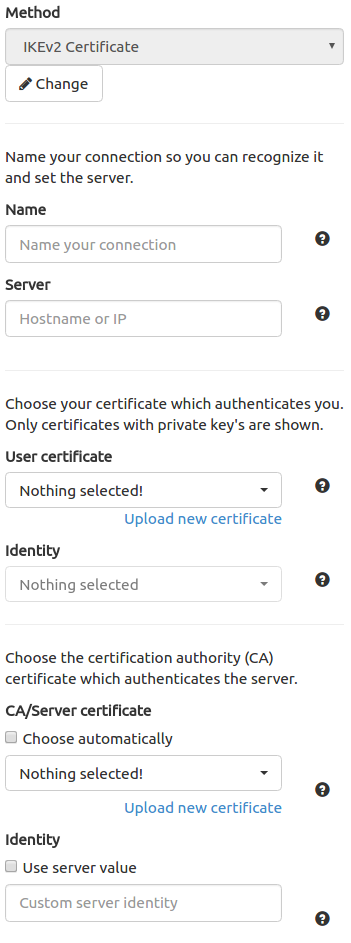
\includegraphics[width=200pt]{images/ike_cert.png}
    	\caption{IKEv2 Certificate}
    \end{figure}
\end{minipage}
\hfill
\begin{minipage}[t]{0.5\textwidth}
\vspace{0pt}
\paragraph{Beschreibung}\mbox{}\\
\paragraph{Name}\label{name}\mbox{}\\
\hspace*{18pt}Ordered Dictionary: 'Bezeichner'\\
Eindeutige Bezeichnung für die Verbindung \\

\paragraph{Server}\label{server}\mbox{}\\
\hspace*{18pt}Ordered Dictionary: remote\_addrs\\
Hostname oder IP des Servers\\

\paragraph{User certificate}\label{usercertificate}\mbox{}\\
\hspace*{18pt}Ordered Dictionary: local.certs\\
Auswahl der Benutzerzertifikate. Im ordered Dictionary wird der komplette DER-Container in Binärer Form übermittelt.\\

\paragraph{Identitiy}\label{identitiy}\mbox{}\\
\hspace*{18pt}Ordered Dictionary: local.id\\
Auswahl zwischen Subject Alternative Name und Distinguished Name. Standardmässig wird der Distinguished Name gesetzt, somit wird nur bei Auswahl eines Subject Alternative Name die local.id in das ordered Dictionary geschrieben.\\

\paragraph{CA/Server certificate}\label{servercertificate}\mbox{}\\
\hspace*{18pt}Ordered Dictionary: remote.cacerts\\
Die automatische Auswahl bewirkt, dass alle CA/Server Zertifikate an den strongSwan übergeben werden und dieser selbständig entscheidet. Ansonsten wird das passende manuell ausgewählt.\\

\paragraph{Server identity}\label{serveridentitiy}\mbox{}\\
\hspace*{18pt}Ordered Dictionary: remote.id\\
Bezeichner für die Serveridentifikation. Per Default wird der \textbf{Server} Eintrag übernommen. Ansonsten auch manuell setzbar.\\

\end{minipage}
\newpage
\subsubsection{IKEv2 Certificate ordered Dictionaries}
\noindent\begin{minipage}[t]{0.5\textwidth}
\vspace{0pt}
\paragraph{Client}\mbox{}\medskip
\begin{lstlisting}[style=BashInputStyle]
{
    "cert": {
        "remote_addrs": [
            "gateway"
        ],
        "vips": [
            "0.0.0.0",
            "::"
        ],
        "version": 2,
        "proposals": [
            "default"
        ],
        "children": {
            "cert": {
                "remote_ts": [
                    "::/0",
                    "0.0.0.0/0"
                ],
                "esp_proposals": [
                    ''aes128gcm128-
                    modp2048''
                ]
            }
        },
        "local": {
            "round": 1,
            "auth": "pubkey"
            "certs": [
                "b'bytes_of_cert'"
            ]
        },
        "remote-cert": {
            "round": 1,
            "auth": "pubkey",
            "id": "moon.strongswan.org"
            "cacerts": [
                "b'bytes_of_cert'"
            ]
        }
    }
}
\end{lstlisting}
\end{minipage}
\hfill
\begin{minipage}[t]{0.5\textwidth}
\vspace{0pt}
\paragraph{Server}\mbox{}\medskip
\begin{lstlisting}[style=BashInputStyle]
{
    "server-cert": {
        "pools": [
            "server-pool"
        ],
        "local": {
            "auth": "pubkey",
            "id": "moon.strongswan.org",
            "certs": [
                "moonCert.pem"
            ]
        },
        "remote": {
            "auth": "pubkey"
        },
        "version": 2,
        "proposals": [
            "aes128-sha256-modp2048"
        ],
        "children": {
            "server-cert": {
                "esp_proposals": [
                    ''aes128gcm128-
                    modp2048''
                ]
            }
        }
   }
}
\end{lstlisting}
\hspace*{18pt}\textbf{Pools}\mbox{}\medskip
\begin{lstlisting}[style=BashInputStyle]
"server-pool": {
    "addrs": "10.6.0.0/24"
}
\end{lstlisting}
\end{minipage}
\newpage



\subsubsection{IKEv2 EAP (Username/Password)}
Die Authentisierung zwischen Client und Server findet auf Basis von EAP mit Hilfe eines Benutzernamens und Passwortes statt.
Die \textbf{eap-id} ist eine Referenz auf das Secret.

\noindent\begin{minipage}[t]{0.5\textwidth}
\vspace{0pt}
\paragraph{Eingabefelder}\mbox{}\medskip
    \begin{figure}[H]
    	\centering
    	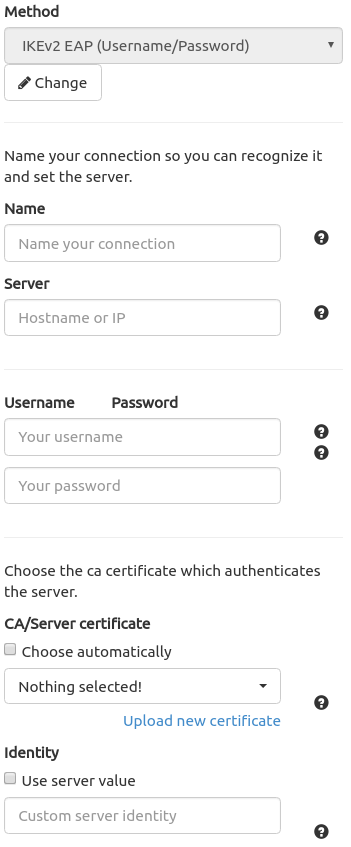
\includegraphics[width=200pt]{images/ike_eap.png}
    	\caption{IKEv2 EAP}
    \end{figure}
\end{minipage}
\hfill
\begin{minipage}[t]{0.5\textwidth}
\vspace{0pt}
\paragraph{Beschreibung}\mbox{}\\

\paragraph{Name}\mbox{}\\
Siehe Seite \pageref{name} \\

\paragraph{Server}\mbox{}\\
Siehe Seite \pageref{server} \\

\paragraph{Username}\label{username}\mbox{}\\
\hspace*{18pt}Ordered Dictionary: secrets.id, local.eap\_id\\
Username wird als als Referenz zwischen den Secrets und der local Section verwendet. \\

\paragraph{Password}\label{password}\mbox{}\\
\hspace*{18pt}Ordered Dictionary: secrets.data\\
Das Passwort für die EAP Authentisierung, es wird verschlüsselt in der Datenbank gespeichert und muss sowohl auf Server-, wie auch Clientseite gesetzt sein.\\

\paragraph{CA/Server certificate}\mbox{}\\
Siehe Seite \pageref{servercertificate} \\

\paragraph{Server identity}\mbox{}\\
Siehe Seite \pageref{serveridentitiy} \\

\end{minipage}
\newpage

\subsubsection{IKEv2 EAP (Username/Password) ordered Dictionaries}
\noindent\begin{minipage}[t]{0.5\textwidth}
\vspace{0pt}
\paragraph{Client}\mbox{}\medskip
\begin{lstlisting}[style=BashInputStyle]
{
    "eap": {
        "remote_addrs": [
            "gateway"
        ],
        "vips": [
            "0.0.0.0",
            "::"
        ],
        "version": 2,
        "proposals": [
            "default"
        ],
        "children": {
            "eap": {
                "remote_ts": [
                    "::/0",
                    "0.0.0.0/0"
                ],
                "esp_proposals": [
                    ''aes128gcm128-
                    modp2048''
                ]
            }
        },
        "local-eap": {
            "round": 1,
            "auth": "eap",
            "eap_id": "eap-test"
        },
        "remote-cert": {
            "round": 1,
            "auth": "pubkey",
            "id": "moon.strongswan.org"
        }
    }
}
\end{lstlisting}
\hspace*{18pt}\textbf{Secrets}\mbox{}\medskip
\begin{lstlisting}[style=BashInputStyle]
{
    "data": "test",
    "id": "eap-test",
    "type": "EAP"
}
\end{lstlisting}
\end{minipage}
\hfill
\begin{minipage}[t]{0.5\textwidth}
\vspace{0pt}
\paragraph{Server}\mbox{}\medskip
\begin{lstlisting}[style=BashInputStyle]
{
    "server-eap": {
        "pools": [
            "server-pool"
        ],
        "local": {
            "auth": "pubkey",
            "id": "moon.strongswan.org",
            "certs": [
                "moonCert.pem"
            ]
        },
        "remote-eap": {
            "auth": "eap-md5"
        },
        "version": 2,
        "proposals": [
            "aes128-sha256-modp2048"
        ],
        "children": {
            "server-eap": {
                "esp_proposals": [
                    ''aes128gcm128-
                    modp2048''
                ]
            }
        }
   }
}
\end{lstlisting}
\hspace*{18pt}\textbf{Secrets}\mbox{}\medskip
\begin{lstlisting}[style=BashInputStyle]
{
    "data": "test",
    "id": "eap-test",
    "type": "EAP"
}
\end{lstlisting}
\hspace*{18pt}\textbf{Pools}\mbox{}\medskip
\begin{lstlisting}[style=BashInputStyle]
"server-pool": {
    "addrs": "10.6.0.0/24"
}
\end{lstlisting}
\end{minipage}


\subsubsection{IKEv2 EAP-TLS}
Mit der EAP-TLS Konfiguration wird ohne separate IKEv2 Authentifikation ein Verbindung aufgebaut, die das TLS Client- und Serverzertifikat verwendet.\\


\noindent\begin{minipage}[t]{0.5\textwidth}
\vspace{0pt}
\paragraph{Eingabefelder}\mbox{}\medskip
    \begin{figure}[H]
    	\centering
    	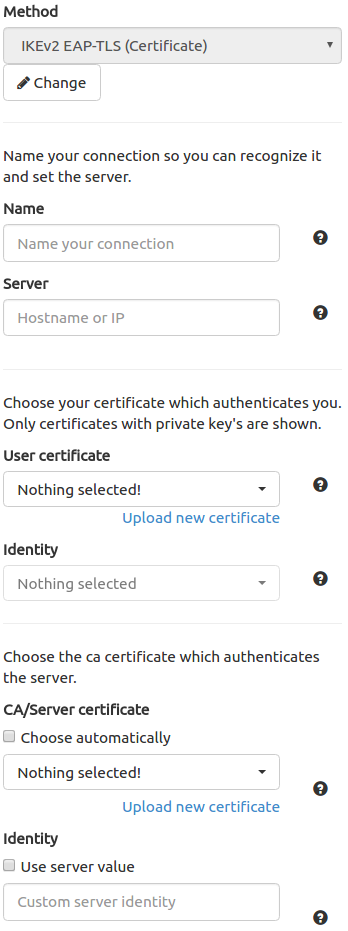
\includegraphics[width=200pt]{images/ike_eap_tls.png}
    	\caption{IKEv2 EAP-TLS}
    \end{figure}
\end{minipage}
\hfill
\begin{minipage}[t]{0.5\textwidth}
\vspace{0pt}
\paragraph{Beschreibung}\mbox{}\\
\paragraph{Name}\mbox{}\\
Siehe Seite \pageref{name} \\

\paragraph{Server}\mbox{}\\
Siehe Seite \pageref{server} \\

\paragraph{CA/Server certificate}\mbox{}\\
Siehe Seite \pageref{servercertificate} \\

\paragraph{Server identity}\mbox{}\\
Siehe Seite \pageref{serveridentitiy} \\

\end{minipage}
\newpage

\subsubsection{IKEv2 EAP-TLS ordered Dictionaries}
\noindent\begin{minipage}[t]{0.5\textwidth}
\vspace{0pt}
\paragraph{Client}\mbox{}\medskip
\begin{lstlisting}[style=BashInputStyle]
{
    "eap-tls": {
        "remote_addrs": [
            "gateway"
        ],
        "vips": [
            "0.0.0.0",
            "::"
        ],
        "version": 2,
        "proposals": [
            "default"
        ],
        "children": {
            "eap-tls": {
                "remote_ts": [
                    "::/0",
                    "0.0.0.0/0"
                ],
                "esp_proposals": [
                    ''aes128gcm128
                    -modp2048''
                ]
            }
        },
        "local-eap-tls": {
            "round": 1,
            "auth": "eap-tls",
            "eap_id": "eap-test"
        },
        "remote-cert": {
            "round": 1,
            "auth": "pubkey",
            "id": "moon.strongswan.org"
        }
    }
}
\end{lstlisting}
\hspace*{18pt}\textbf{Secrets}\mbox{}\medskip
\begin{lstlisting}[style=BashInputStyle]
{
    "data": "test",
    "id": "eap-test",
    "type": "EAP"
}
\end{lstlisting}
\end{minipage}
\hfill
\begin{minipage}[t]{0.5\textwidth}
\vspace{0pt}
\paragraph{Server}\mbox{}\medskip
\begin{lstlisting}[style=BashInputStyle]
{
    "server-eap-tls": {
        "pools": [
            "server-pool"
        ],
        "local": {
            "auth": "pubkey",
            "id": "moon.strongswan.org",
            "certs": [
                "moonCert.pem"
            ]
        },
        "remote-eap": {
            "auth": "eap-dynamic"
            "eap_id": "eap-test"
        },
        "version": 2,
        "proposals": [
            "aes128-sha256-modp2048"
        ],
        "children": {
            "server-eap-tls": {
                "esp_proposals": [
                    ''aes128gcm128-
                    modp2048''
                ]
            }
        }
   }
}
\end{lstlisting}
\hspace*{18pt}\textbf{Secrets}\mbox{}\medskip
\begin{lstlisting}[style=BashInputStyle]
{
    "data": "test",
    "id": "eap-test",
    "type": "EAP"
}
\end{lstlisting}
\hspace*{18pt}\textbf{Pools}\mbox{}\medskip
\begin{lstlisting}[style=BashInputStyle]
"server-pool": {
    "addrs": "10.6.0.0/24"
}
\end{lstlisting}
\end{minipage}
\newpage


\subsubsection{IKEv2 Certificate + EAP (Username/Password)}
Zwei Runden Authentisierung, basierend auf der Kombination von EAP und Zertifikat.\\

\noindent\begin{minipage}[t]{0.5\textwidth}
\vspace{0pt}
\paragraph{Eingabefelder}\mbox{}\medskip
    \begin{figure}[H]
    	\centering
    	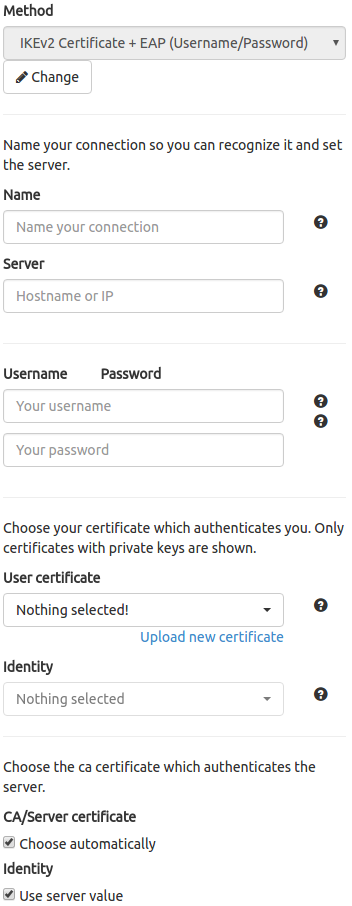
\includegraphics[width=200pt]{images/ike_cert_eap.png}
    	\caption{IKEv2 Certificate + EAP}
    \end{figure}
\end{minipage}
\hfill
\begin{minipage}[t]{0.5\textwidth}
\vspace{0pt}
\paragraph{Beschreibung}\mbox{}\\
\paragraph{Name}\mbox{}\\
Siehe Seite \pageref{name} \\

\paragraph{Server}\mbox{}\\
Siehe Seite \pageref{server} \\

\paragraph{Username}\mbox{}\\
Siehe Seite \pageref{username} \\

\paragraph{Password}\mbox{}\\
Siehe Seite \pageref{password} \\

\paragraph{CA/Server certificate}\mbox{}\\
Siehe Seite \pageref{servercertificate} \\

\paragraph{Server identity}\mbox{}\\
Siehe Seite \pageref{serveridentitiy} \\

\end{minipage}
\newpage

\subsubsection{IKEv2 Certificate + EAP (Username/Password) ordered Dictionaries}
\noindent\begin{minipage}[t]{0.5\textwidth}
\vspace{0pt}
\paragraph{Client}\mbox{}\medskip
\begin{lstlisting}[style=BashInputStyle]
{
    "eap-cert": {
        "remote_addrs": [
            "gateway"
        ],
        "vips": [
            "0.0.0.0",
            "::"
        ],
        "version": 2,
        "proposals": [
            "aes128-sha256-modp2048"
        ],
        "children": {
            "eap-cert": {
                "remote_ts": [
                    "::/0",
                    "0.0.0.0/0"
                ],
                "esp_proposals": [
                    ''aes128gcm128-
                    modp2048''
                ]
            }
        },
        "local-cert": {
            "round": 1,
            "auth": "pubkey"
        },
        "local-eap": {
            "round": 2,
            "auth": "eap",
            "eap_id": "eap-test"
        },
        "remote-eap-cert": {
            "round": 1,
            "auth": "pubkey",
            "id": "moon.strongswan.org"
        }
    }
}
\end{lstlisting}
\hspace*{18pt}\textbf{Secrets}\mbox{}\medskip
\begin{lstlisting}[style=BashInputStyle]
{   "data": "test",
    "id": "eap-test",
    "type": "EAP"   }
\end{lstlisting}
\end{minipage}
\hfill
\begin{minipage}[t]{0.5\textwidth}
\vspace{0pt}
\paragraph{Server}\mbox{}\medskip
\begin{lstlisting}[style=BashInputStyle]
{
    "server-cert-eap": {
        "pools": [
            "server-pool"
        ],
        "local": {
            "auth": "pubkey",
            "id": "moon.strongswan.org",
            "certs": [
                "moonCert.pem"
            ]
        },
        "remote": {
            "auth": "pubkey",
            "round": 1
        },
        "remote-eap": {
            "auth": "eap-md5",
            "eap_id": "eap-test",
            "round": 2
        },
        "version": 2,
        "proposals": [
            "aes128-sha256-modp2048"
        ],
        "children": {
            "server-cert-eap": {
                "esp_proposals": [
                    ''aes128gcm128-
                    modp2048''
                ]
            }
        }
   }
}
\end{lstlisting}
\hspace*{18pt}\textbf{Secrets}\mbox{}\medskip
\begin{lstlisting}[style=BashInputStyle]
{   
    "data": "test",
    "id": "eap-test",
    "type": "EAP"   
}
\end{lstlisting}
\hspace*{18pt}\textbf{Pools}\mbox{}\medskip
\begin{lstlisting}[style=BashInputStyle]
"server-pool": {
    "addrs": "10.6.0.0/24"
}
\end{lstlisting}
\end{minipage}
\nolinebreak
\nopagebreak